%-------------------------------------------------------------------------------------------------%
% A related work section in which the relevant literature is presented and 
% linked to the project. 
% It should show that you clearly know the problem you plan to solve, 
% and that you master the related work. 
\newpage

\section{Related work}

This chapter offers background literature on the aforementioned topics, and will explain how this literature relates to the proposed study. three related topics are regarded: prior studies on WebAssembly, Prior studies on client-side geoprocessing, and prior studies on geoprocessing interfaces.


\subsection{WebAssembly \& Geoprocessing performance}

% Why are you writing this? 

On 5 December 2019, the \ac{w3c} officially pronounced WebAssembly as the fourth programming language of the web \cite{w3c_world_2019}. Philippe Le Hégaret, the \ac{w3c} Project Lead, writes “The arrival of WebAssembly expands the range of applications that can be achieved by simply using Open Web Platform technologies. In a world where machine learning and Artificial Intelligence become more and more common, it is important to enable high performance applications on the Web, without compromising the safety of the users,”. Since then, most major browsers have added WebAssembly support.

To the best of the author's knowledge, and as of writing this proposal, no papers explicitly links WebAssembly and Geodata processing. The original paper paper on \ac{wasm} does state \textit{3d data processing} as one of the examples for high performance web applications \cite{haas_bringing_2017}.. What's more, Google Earth uses WebAssembly as seen in \reffig{fig:google-earth} \cite{google_google_2020}. How it is used is unknown due to the engine being closed-source, but it is speculated that \ac{wasm} is used to access code written for the original C++-based desktop application.


\cite{jangda_not_2019, haas_bringing_2017}.

\begin{figure}[!tbp]
  \centering
  \begin{minipage}[b]{0.80\textwidth}
    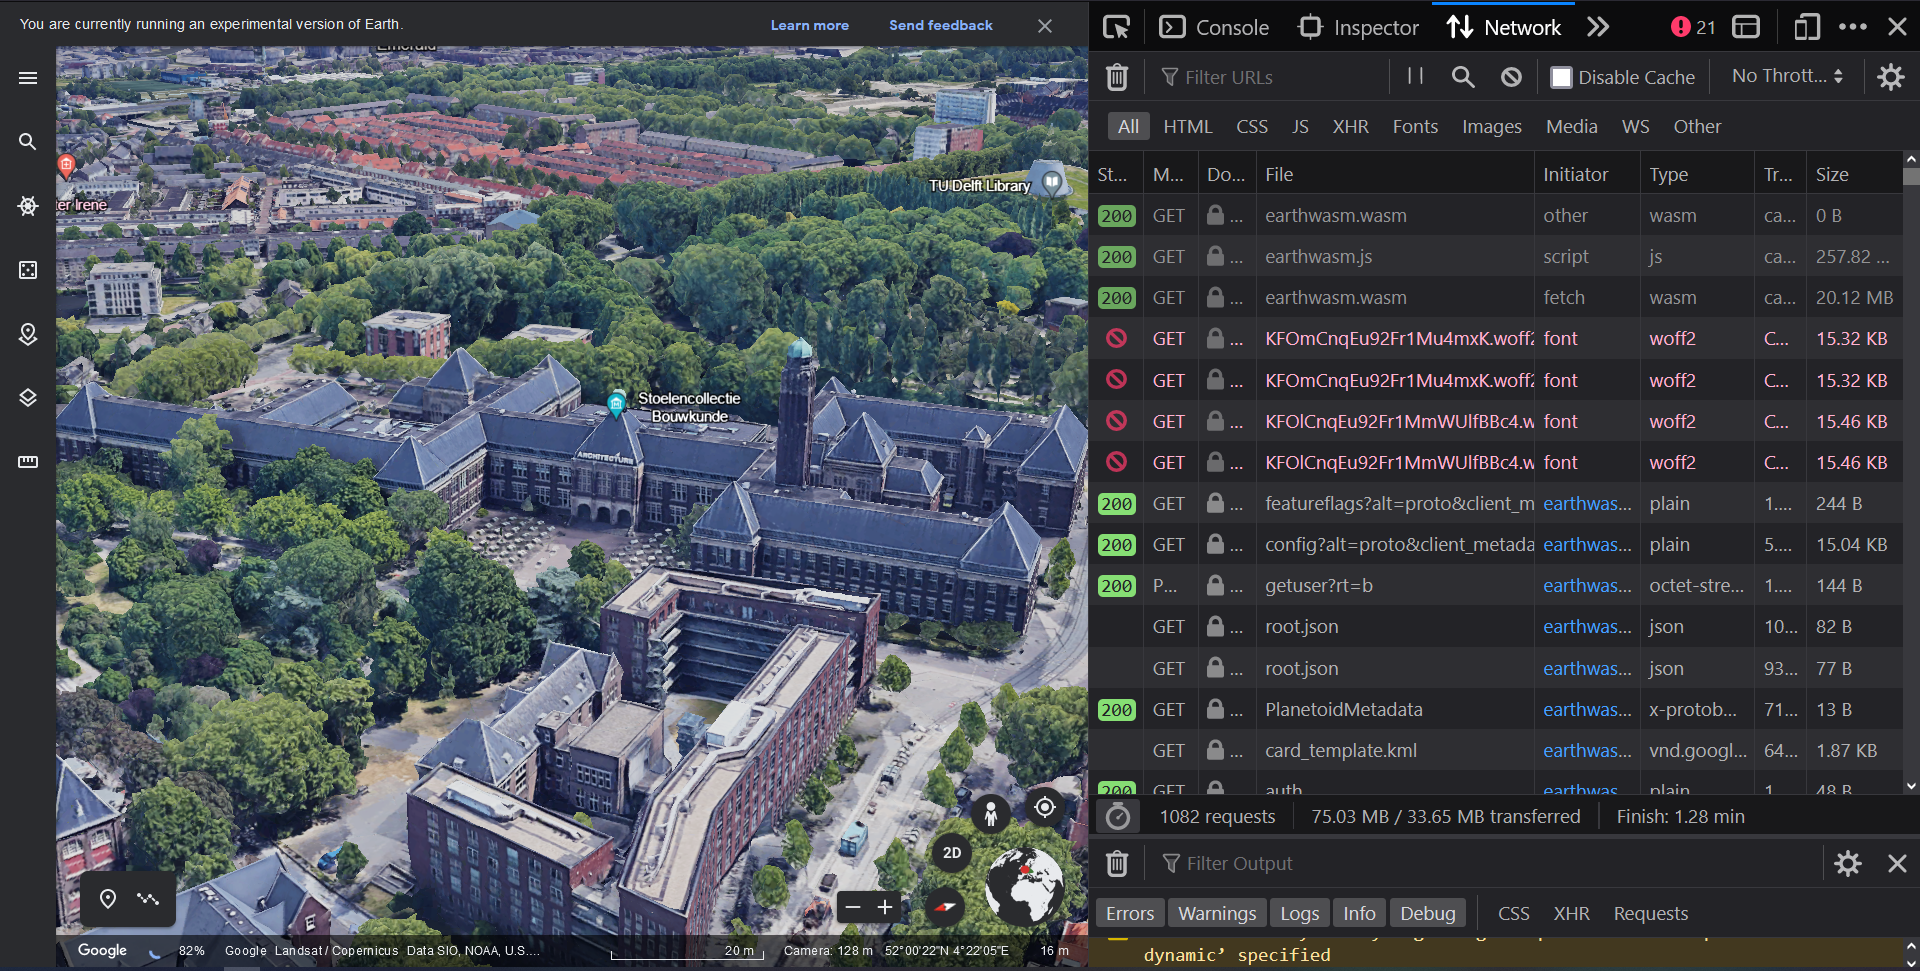
\includegraphics[width=\textwidth]{../images/google-earth-uses-webassembly.PNG}
    \caption{Google Earth utilizing WebAssembly. Source: \cite{google_google_2020}}
    \label{fig:google-earth}
  \end{minipage}
\end{figure}



The performance benefits of using WebAssembly for other purposes than geoprocessing have seen prior study. \cite{jangda_not_2019}.



% ORIGINAL PAPER

% ### x.x.x Bringing the Web up to Speed with WebAssembly
% This is the original paper introducing WebAssembly in 2017, co-written by software engineers from the major browser vendors Mozilla, Google, Apple and Microsoft. 
% It defines that a low-level compilation target should be
% save, fast, portable and compact.
% It continues by showing how previous attempts at low-level code on the web fail in at least one of these criteria, and that WebAssembly is the first to delivers on all of them. 
% The chapters following this up cover the design details of the language, and the decisions which had to be made to live up to the four criteria. 
% These details will become relevant when reasoning about why WebAssembly might be faster in one case versus another.
% <!-- proof of memory savety, proof of soundness  -->

% <!-- EXPLORE TYPES & EFFICIENT LOADING OF DATA TYPES BETWEEN UNRELATED LIBRARIES -->

% Chapter 6 and 7 also require special attention.
% Chapter 6 shows the possibilities available to a host environment for compiling, instantiating and invoking wasm binaries. 


% Chapter 7 : Implementation: 
% - validate
% - execution time
% - binary size 

% Initial benchmarks look promising
% large portion of benchmarks within 10% 

% <!-- 
% Interoperability It is possible to link multiple modules that
% have been created by different producers. However, as a low-
% level language, WebAssembly does not provide any built-in
% object model. It is up to producers to map their data types
% to numbers or the memory. This design provides maximum
% flexibility to producers, and unlike previous VMs, does not
% privilege any specific programming or object model while
% penalizing others. Though WebAssembly has a program-
% ming language shape, it is an abstraction over hardware, not
% over a programming language.
% Interested producers can define common ABIs on top of
% WebAssembly such that modules can interoperate in hetero-
% geneous applications. This separation of concerns is vital for
% making WebAssembly universal as a code format -->

%%%%%%%%%%%%%%%%%%%%%%%%%%%%%%%%%%%%%%%%%%%%%%%%%%%%%%%%%%%%%%%%%%%%%%%%%%%%%%%

% Not So Fast WebAssembly Paper 

% Paper exploring performance of WebAssembly more thorough.

% Starts out positive: current benchmarks (2019) are even better than those of the original paper (2017). 

% BUT 

% Those original papers cover a type of benchmark which uses mainly scientific operations as benchmarks. 
% Each of these operations are roughly 100 lines of code.
% This paper created a way to compile full, large-scale applications into WebAssembly, and proceeds to benchmark them. 
% They found that these types of applications run significantly slower and spikier.

% BUT 

% This might not be a problem for the scope of this research. 
% This research will deal with the originally criticized scientific purposes anyway.
% If it does turn out that wasm performs significantly slower the larger the binaries are, This research might explore disecting the C++ libraries into a number of tiny wasm Binaries, one per function for example, or per .cpp file. 
% As stated in the Wasm paper (SOURCE), it is possible to inject precompiled wasm binaries within other wasm binaries. 
% This way, the functionalities of one library could be lazy-initialized, so only the parts that are necessairy are being compiled and used. 
% Food for thought...

% ...

% A telling example of the cause of the loss in speed is this: 

% NATIVE: 
% C --{CLANG}-> x86-64 code

% WEB
% C --{EMSC}-> WASM --{JIT}-> x86-64 code 

% + Chapter 6 is very significant

% <!-- 6.4 Discussion
% It is worth asking if the performance issues identified here
% are fundamental. We believe that two of the identified is-
% sues are not: that is, they could be ameliorated by improved
% implementations. WebAssembly implementations today use
% register allocators (§6.1.2) and code generators (§6.2.1) that
% perform worse than Clang’s counterparts. However, an offline
% compiler like Clang can spend considerably more time to
% generate better code, whereas WebAssembly compilers must
% be fast enough to run online. Therefore, solutions adopted
% by other JITs, such as further optimizing hot code, are likely
% applicable here [19, 32].
% The four other issues that we have identified appear to
% USENIX Association 2019 USENIX Annual Technical Conference    117
% arise from the design constraints of WebAssembly: the stack
% overflow checks (§6.2.2), indirect call checks (§6.2.3), and
% reserved registers (§6.1.1) have a runtime cost and lead to in-
% creased code size (§6.3). Unfortunately, these checks are nec-
% essary for WebAssembly’s safety guarantees. A redesigned
% WebAssembly, with richer types for memory and function
% pointers [23], might be able to perform some of these checks
% at compile time, but that could complicate the implementa-
% tion of compilers that produce WebAssembly. Finally, a Web-
% Assembly implementation in a browser must interoperate with
% a high-performance JavaScript implementation, which may
% impose its own constraints. For example, current JavaScript
% implementations reserve a few registers for their own use,
% which increases register pressure on WebAssembly. -->

% <!-- 
% WHY PERFORMANCE LOST: LOST IN TRANSLATION 

% NATIVE: 
% C --{CLANG}-> x86-64 code

% WEB
% C --{EMSC}-> WASM --{JIT}-> x86-64 code 

% Seems to be

%  -->


% <!-- 

% TODO
% look into the specifics of the benchmarks provided 
% PolyBenchC seems to contain a lot of geometry operatinos, which seems good news for us



% SIGNIFICANT FOR GEOMATICS: 
% sync I/O is hard to do with webassembly. This could be detremental for many geomatics applciations



% The standard approach to running these applications today
% is to use Emscripten, a toolchain for compiling C and C++ to
% WebAssembly [39]. Unfortunately, Emscripten only supports
% the most trivial system calls and does not scale up to large-
% scale applications. For example, to enable applications to use
% synchronous I/O, the default Emscripten MEMFS filesystem
% loads the entire filesystem image into memory before the
% program begins executing. For SPEC, these files are too large
% to fit into memory

%  -->






\subsection{On client-side geoprocessing}

Client-side, browser based geoprocessing has seen academic interested throughout the last decade. 

- 

- timely nature

- performance 


% ### x.x.x 2014 Client-side versus Server-side Geoprocessing ...

% *These results demonstrated that the current implementation of web browsers are limited in their ability to execute JavaScript geoprocessing and not yet prepared to process data sizes larger than about 7,000 to 10,000 vertices before either prompting an unresponsive script warning in the browser or potentially losing the interest of the user.*

% This paper is very similar to what i'm doing, and it makes a conclusion that scared me at first glance. Then I saw that this is a paper out of 2014.

% The results of this paper are insightful, but do not directly applicable to this paper because of three reasons: 
% 1. The paper used javascript-based geoprocessing, not `asm.js` optimized. This is known to be inefficient. 
% 2. The paper stems from 2014. is before an incredible industry-wide performance increase of javascript interpreters. 
%    This is the result of technological development in the form of an arms race between the major browswer vendors. 
% 3. This paper will introduce WebAssembly to speed things up. 


%%%%%%%%%%%%%%%%%%%%%%%%%%%%%%%%%%%%%%%%%%%%%%%%%%%%%%%%%%%%%%%%%%%%%%%%%%%%%%%


% ### x.x.x Hybrid Geoprocessing Web Services

% This paper proposes a hybrid strategy, using the OGC Web Processing services as a starting point, and building client-side tools around it. This is different from the approach offered by this study, which starts from the well-known CGAL and GDAL geoprocessing libraries. The environment proposed by this thesis might offer OGC Web Processing services, inspired by this paper. 


%%%%%%%%%%%%%%%%%%%%%%%%%%%%%%%%%%%%%%%%%%%%%%%%%%%%%%%%%%%%%%%%%%%%%%%%%%%%%%%


% ### x.x.x Analysis of server-side and client-side Web-GIS data processing methods on the example of JTS and JSTS using open data from OSM and geoportal

% <!-- The last decade has seen a rapid evolution of processing, analysis and visualization of freely available geographic data using Open Source Web-GIS. In the beginning, Web-based Geographic Information Systems employed a thick-client approach which required installation of platform-specific browser plugins. Later on, research focus shifted to platform-independent thin client solutions in which data processing and analysis was performed by the server machine. More recently, however, the rapid development of computer hardware as well as software technologies such has HTML5 has enabled the creation of platform-independent thick clients which offer advanced GIS functionalities such as geoprocessing. This article aims to analyse the current state of Open Source technologies and publicly available geographic data sources in the context of creating cost-effective Web-GIS applications for integration and processing of spatial data. For this purpose the article discusses the availability and potential of Web-GIS architectures, software libraries and data sources. The analysis of freely available data sources includes a discussion of the quality and accuracy of crowd-sourced as well as public sector data, while the investigation of software libraries and architectures involves a comparison of server-side and client-side data processing performance under a set of real-world scenarios. The article concludes with a discussion of the choice of cost-effective Web-GIS architectures, software libraries and data sources in the context of the institution and environment of system deployment. -->

% This is a very relevant source




\subsection{On geoprocessing interfaces}

Finally, this proposal wishes to examine the state of the art of studies regarding geoprocessing interfaces. Unfortunately, most studies concerned specifically with geodata processing interfaces have a one to one relationship between application and interface. most papers do not state general user interface principles. At the same time, general UI studies are too broad, and while insightful, the scope is too big. 

Therefore, we stay close to home, and instead base interface considerations on

topic SDI research \& geoweb

interesting links can be made between

A noteworthy paper on this topic is Van den Brink's phd titled "Geospatial Data on the Web". Van den Brink states that geodata remains useful exclusively to experts in the field, despite all efforts to improve accessibility. 
She then presents the case for opening up geodata to a wider audience and more communities: "An important set of present-day users can be called “data users”: web developers, data journalists etc. who use different kinds of data, including geospatial data, directly to create applications or visualizations that supply information to end users (citizens). In order to achieve the wide re-use of geospatial data across communities, data should be easily accessible by these data users.". She also mentions the concept of FAIR geodata. Coined by \cite{mark_d_wilkinson_fair_2016}, The FAIR principles are a collection of four well-established assessment criteria used for judging the usability of data: Findable, Accessible, Interoperable, and Reusable. 

The proposed thesis acknowledges these concerns, and proposes to extend the concept of FAIR geodata to geoprocessing as well. This thesis therefore aims to make its proposed software as Findable, Accessible, Interoperable, and Reusable as possible. 

It is for these reasons that the topic of user interface will be part of this thesis. 

UI : as Findable, Accessible, Interoperable, and Reusable as possible. 

open, cross community, base on both web, w3c standards and OGC.

for these reasons, VPL chosen, so even non-programmers



- Ravi?

Lots of research has been done on the topic of VPL's, and their advantages and disadvantages. 
(I explicitly want to name the cognitive dimentions paper, it is very good and appropriate, and contains many suggestions for future VPL's)


% WebAssembly has the potential to improve all four of those criteria for software. If an application is published on the web without login requirements, makes it so there is no difference between Findability and Accessibility. As soon as it can be found, it can be accessed. 

% Additionally, \ac{wasm} is created explicitly to make software more \textit{Interoperable} and \textit{Reusable}.
% A ac{wasm} compiled library will work the same, wherever it is run. It is a manifestation of the  
% \textit{Write once, use anywhere} paradigm, not completely unrelated to the \textit{Collect once, use multiple times} paradigm, as both aim to minimize redundancy.



%%%%%%%%%%%%%%%%%%%%%%%%%%%%%%%%%%%%%%%%%%%%%%%%%%%%%%%%%%%%%%%%%%%%%%%%%%%%%%%


To the best of the author's knowledge, no papers exist coupling VPL to geoprocessing.

Still, this is being done, evident by...


Examination of multiple VPLS:






\subsection{Conclusion}

- Time is important 
- 'missing link'


